\documentclass[]{scrartcl}
\usepackage{graphicx}
%\pagestyle{headings}

\begin{document}

\title{Sensory Analysis}
\subtitle{brewing lecture at TU-Berlin}
\author{Christopher Weyand}
\maketitle
\begin{abstract}
Brewing is a widespread field including the scientific disciple of sensory analysis
that, for the purpose of evaluating consumer products, applies principles of experimental
design and statistical analysis to the use of human senses.
\end{abstract}
\newpage

\tableofcontents
\newpage

\listoffigures
\newpage

\section{Main Goals}
\begin{enumerate}
  \item Comparison
  \item Description
  \item Preference
\end{enumerate}


\section{Definition of Sensory Analysis}
A sensory evaluation is performed to detect, identify and evaluate
characteristics of products utilizing all of the sensory pathways.
(olfactory, visual, gustatory, auditory, tactile)


\section{tactile analysis}
\begin{itemize}
  \item tingling
  \item viscosity
  \item temperature
\end{itemize}


\section{Testing Methods}
Below follows a section about the methods of sensory testing in scientific environments.
They are listed in alphabetical order.
\subsection{authenticity test}
Does the product meet customer expectations.

\subsection{aversion test}
This test is a prederence test that permits just like or dislike as an answer.

\subsection{blind test}
The test subjects are left in the dark about the type or brand of the sample.

\subsection{branded test}
The branded test is the counterpart to the blind test.

\subsection{descriptive testing}
QDA: quantitative descriptive analysis

\subsection{difference tests}
Difference tests include the difference ranking test.

\subsection{duo-trio test}
It is to determine with wich of two original samples a third sample matches.

\subsection{hedonic test}
Hedonic or affective tests are simple processes to determine ones preferences offering
just a few options to chose from.

\subsection{monadic test}
The monadic test is done using just one sample and no comparison.

\subsection{threshold test}
//todo

\subsection{time intensity test}
Refers to the behavior of sensory impressions like bitter -or tardness over time
as seen in figure \ref{fig:time-intensity}.
\begin{figure}[h]
	\centering
	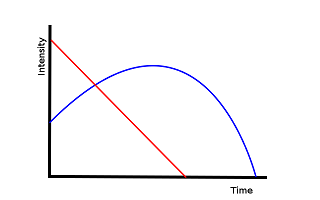
\includegraphics{time-intensity.png}
	\caption{intensity of sensory impression over time}
	\label{fig:time-intensity}
\end{figure}

\subsection{triangle test}
//todo

\newpage
\section{Miscellaneous}
Before Sensorik you shall not:
\begin{itemize}
  \item smoke
  \item eat chocolate
  \item use perfume
  \item forget to shower
\end{itemize}
Also women are more sensitive to olfactory impulses. Furthermore they gustatory perceive
more intense in special ways including the bitterness. This leads to aversion of bitter beer
by most women.

\end{document}
